\section{Odds \& Ends}

\subsection{Ellipse, Locus Range, and Animation Background} 

As shown in  \cref{fig:09-ellipse-range}, the area immediately below the four sets channel controls the following parameters:

\begin{itemize}
    \item \texttt{ell} checkbox: whether the main ellipse underlying a triangle family of choice should be drawn or not.
    \item Rotation menu: the default \texttt{rot off} setting leaves the animation window as is. Settings  \texttt{$90^\circ$,$180^\circ$,$270^\circ$} apply a global rotation to the picture drawn.
    \item \texttt{rmax} menu: the (half-side) of the square bounding box where points in all loci are evaluated, respective to the minor semi-axis of the ellipse, assume to be of unit length. Ideally, this should be set to as small a value as able to contain all loci. 
    \item \texttt{bg}: used to set the background color of the main animation window, dark blue by default. By clicking on the colored square an RGB picker window pops-up permitting fine control of the color.
    \item \texttt{invert} button: single-click inversion (in RGB space) of colors of background and loci currently in being drawn.
\end{itemize}

\begin{figure}
    \centering
    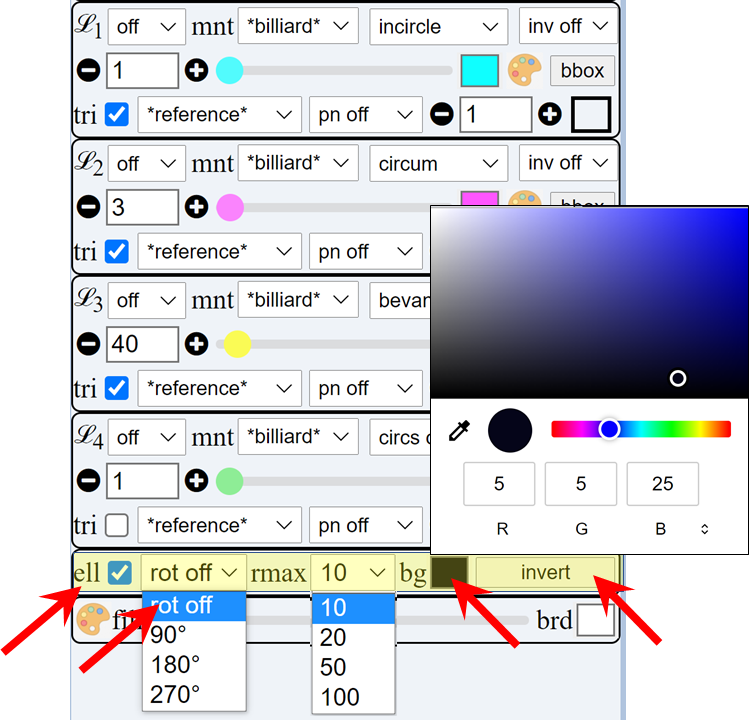
\includegraphics[width=.8\textwidth]{pics_09_140_animation_appearance.png}
    \caption{In the highlighted area controls are available to (i) \texttt{ell}: show or hide the main ellipse, (ii) \texttt{rot xxx}: apply a global rotation to the animation widow, (iii) \texttt{rmax}: set the bounding box of the area in which loci are computed, (iv) \texttt{bg}: set the animation window's background color, and (v) \texttt{invert}: invert (RGB negative) colors of background and all loci drawn.}
    \label{fig:09-ellipse-range}
\end{figure}

\subsection{Resetting the UI and Recentering the Animation} 

\cref{fig:09-anim-appearance} highlights \texttt{reset UI} and \texttt{center UI} push-buttons are located at the top-left corner of the app. These are used to (i) restore all controls in the app to their default values, and (ii) recenter the geometry drawn to the center of the animation, respectively. 

\subsection{Setting the Locus Color}

Also shown in \cref{fig:09-anim-appearance} are color and rescaling controls to the right of the triangle center scrollbar. These are permit (i) selection of a color specific to a particular locus being drawn, and (ii) a resizing/re-centering of the particular locus so as to best fit the animation window.

\begin{figure}
    \centering
    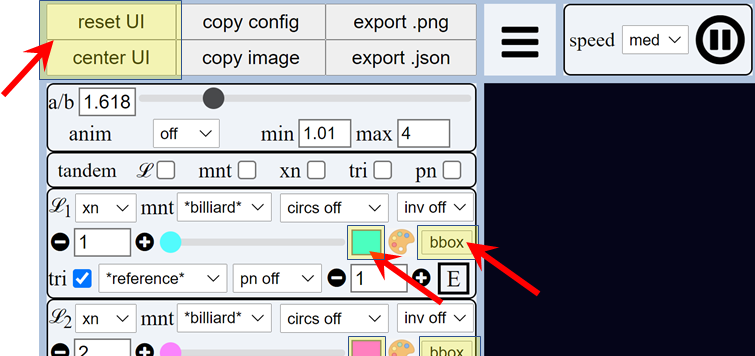
\includegraphics[width=.8\textwidth]{pics_09_150_centering_bbox.png}
    \caption{Reset and center push-buttons are located at the top-left corner of the app.  which (i) \texttt{reset UI}: all controls in the app are restored to their default values; (ii) \texttt{center UI}: the center of the simulation is panned back to the center of the animation area. This is useful after having previously panned the picture via a mouse drag. Also shown is (iii) a color selector square located to the right of every triangle center scrollbar, through which a new color can be selected for displaying the corresponding locus. Finally, (iv) a \texttt{bbox} push button is provided to repositing and scale the geometric scene so as to best fit it in the available space.}
    \label{fig:09-anim-appearance}
\end{figure}

\subsection{Collapsing the Locus Control Area}

The ``hamburger'' control shown in \cref{fig:09-hamburger} can be used to hide/expand the set of controls on the left marging of the app, sometimes useful for demonstration purposes.

\begin{figure}
    \centering
    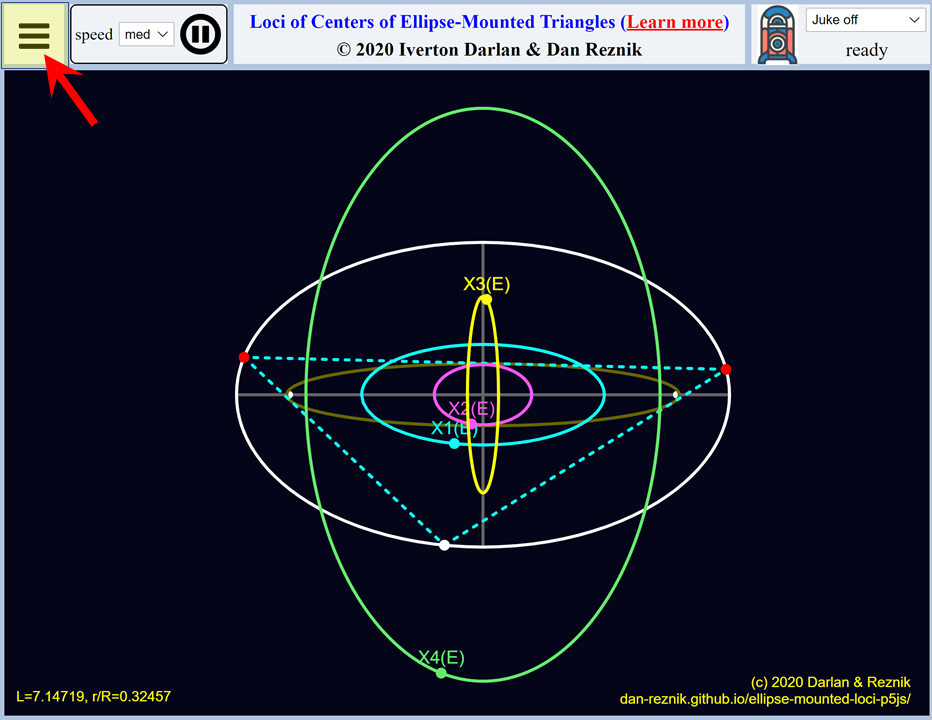
\includegraphics[trim=0 0 150 0,clip,width=.6\textwidth]{pics_09_170_hamburger.png}
    \caption{The hamburger control (three horizontal bars) located to the right of the the main controls can be clicked to hides/expand the main controls.}
    \label{fig:09-hamburger}
\end{figure}